\chapter{Funcionalidades desarrolladas del sistema}
\thispagestyle{empty} % Quitar el número
\glsresetall

En este capítulo se enuncian y describen las funcionalidades desarrolladas en el proyecto de pasantía, así como algunas previas que se relacionen o hayan sido modificadas para facilitar el entendimiento del lector.

Un \gls{SGA} se caracteriza por organizar todas las tareas que faciliten el entendimiento de un concepto por parte de los estudiantes. Entre estas existen cursos, chats, calendarios, estadísticas, etc.

Se debió a lo largo del proyecto implementar el soporte para un nuevo tipo de cursos: los cursos presenciales o seminarios. En los que un nuevo tipo de usuario: el instructor. Dicta una clase presencial sobre un tema que generalmente no puede ser cubierto mediante un curso en línea individual, debido a su complejidad, la importancia de la interacción en grupo para la realización de la actividad, entre otros.

Estos seminarios generalmente se realizan en ubicaciones físicas donde el instructor y los aprendices se encuentran cara a cara, pero también existe la modalidad de conferencias en línea para equipos internacionales.

Los usuarios podrían entonces escoger entre distintas sesiones en las que un seminario puede realizarse. Esto se realiza en respuesta a las limitaciones de tiempo que podría tener un grupo de estudiantes.

Las actividades previamente descritas son administradas por el usuario que toma el rol de administrador en el sistema, que tiene la potestad de crear, modificar y eliminar tanto los cursos como las ubicaciones.

Este relato surge del levantamiento de información realizado mayormente al principio del proyecto, en el que se identificaron las necesidades del cliente para los módulos y que se plasmó formalmente en el Diagrama de Casos de Uso que se muestra a continuación en la figura \ref{fig:diagramaCasosDeUso}.


A continuación, se explican los componentes más importantes presentes en el Diagrama.

	\section{Actores} % (fold)
	\label{sec:usuarios}

	Para el desarrollo de los módulos se requirió de la participación de tres tipos de usuarios, administrador, instructor y aprendiz.
	\begin{figure}[h]
		\begin{center}
			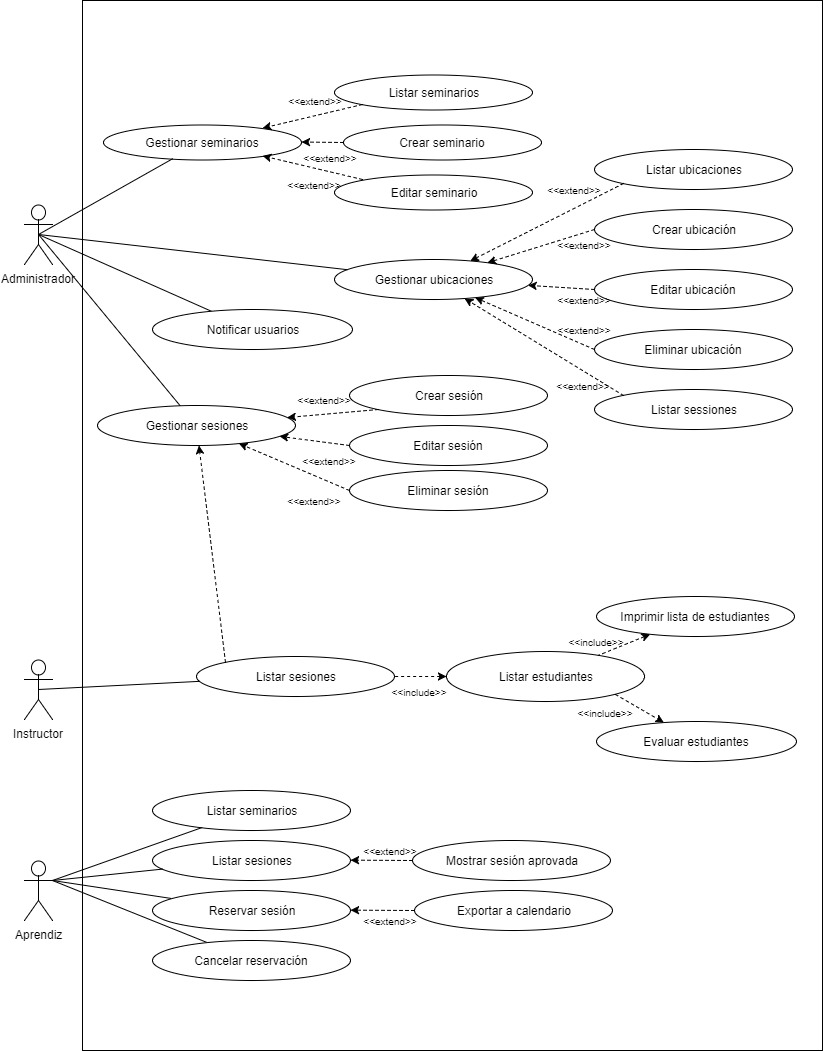
\includegraphics[width=\textwidth]{figuras/diagramaCasosDeUso.jpg}
			\caption{Diagrama de casos de uso.} \label{fig:diagramaCasosDeUso}
		\end{center}
	\end{figure}

		\subsection{Administrador} % (fold)
		\label{sub:administrador}
		
		El usuario administrador se encarga de tres tareas importantes según se visualiza en la figura \ref{fig:diagramaCasosDeUso}. Gestionar los seminarios, las sesiones, las ubicaciones donde éstas se realizan y las notificaciones recibidas por los distintos tipos de usuarios.

			\subsubsection{Gestionar ubicaciones}

			Un módulo de gestión de ubicaciones fue creado para su mejor visualización por medio de un mapa y reúso entre distintas sesiones. El administrador puede crear, editar listar y modificar las ubicaciones que luego serán asignadas a las distintas sesiones. Además, puede especificar la capacidad de las mismas, así como visualizar en un calendario las sesiones planificadas para la misma.

			\subsubsection{Gestionar seminarios}

			Los administradores podrían listar los seminarios, crear un seminario nuevo y asignarlo a grupos de aprendices preestablecidos y por último pueden modificar los datos del mismo.


			\subsubsection{Gestionar sesiones}	
			
			Cada seminario, puede contener una cantidad arbitraria de sesiones, las funcionalidades son parecidas a las que posee sobre los seminarios con la diferencia de que para crear una sesión el administrador asigna un usuario del sistema como instructor, una ubicación preestablecida y fechas de inicio y fin en las que la sesión se realizará.

			Las sesiones pueden ser tanto encuentros físicos como conferencias en línea, cuya diferencia es la asignación del tipo de ubicación.

			\subsubsection{Notificar usuarios}

			Los administradores tienen también la potestad de decidir si las notificaciones de interacción entre los aprendices y los instructores son enviadas o no. Como lo son las notificaciones de confirmación o cancelación por parte de los aprendices, o la cancelación de una sesión no vacía.

		% subsection administrador (end)

		\subsection{Instructor} % (fold)
		\label{sub:instructor}
		
		El usuario instructor es el que se encarga del dictado de una lección, para esto necesita gestionar sus sesiones y manejar las calificaciones de los usuarios. Esta es una de las funciones que puede realizar el administrador a través de la gestión de sesiones.

			\subsubsection{Listar sesiones}

			Un administrador puede listar todas las sesiones de todos los cursos, un instructor solo podrá acceder a las sesiones de las que él sea instructor, valga la redundancia.

			\subsubsection{Imprimir lista de estudiantes}

			El instructor puede imprimir una lista de los usuarios confirmados para la sesión pertinente, con los datos importantes de la misma. 

			\subsubsection{Evaluar estudiantes}

			Dentro del listado de los estudiantes confirmados para una sesión el instructor puede modificar la asistencia, así como indicar la aprobación de un curso por parte de un aprendiz.

		% subsection instructor (end)

		\subsection{Aprendiz} % (fold)
		\label{sub:aprendiz}
		
		Un usuario aprendiz interactúa con los cursos que le han sido asignados, visualiza las ubicaciones y tiene un canal de comunicación con los instructores de las distintas sesiones.

			\subsubsection{Gestionar reservas}
			Un usuario puede listar las sesiones de los distintos cursos que le han sido asignados. Al hacerlo tiene la posibilidad de confirmar su asistencia a la sesión que le parezca más conveniente viendo los instructores, fechas y ubicaciones de cada una. Puede también cancelar una sesión a la que haya confirmado asistencia.

			Además, puede descargar los datos de la sesión y agregarlos directamente a su calendario de preferencia.

			Si el usuario posee una sesión aprobada en un seminario se mostrarán los datos que describan dicha sesión.

		% subsection aprendiz (end)



% section usuarios (end)

